\documentclass[10pt,a4paper]{article}
\usepackage[utf8]{inputenc}
\usepackage{amsmath}
\usepackage{amsfonts}
\usepackage{amsthm}
\usepackage{amssymb}
\usepackage{mathtools}
\DeclarePairedDelimiter\Floor\lfloor\rfloor
\DeclarePairedDelimiter\Ceil\lceil\rceil
\usepackage{listings}
\usepackage{color}
\definecolor{light-gray}{gray}{0.92}
\usepackage{graphicx}
\usepackage[left=2cm,right=2cm,top=2cm,bottom=2cm]{geometry}
\usepackage{relsize}
\usepackage[english]{babel}
\usepackage[utf8]{inputenc}
\usepackage{fancyhdr}
\linespread{1.2}
\pagestyle{fancy}
\fancyhf{}
\rhead{\textit{Joseph High \ \ Hopkins ID: 9E1FDC}}
\lhead{\textit{553.732 (STAT 732) Midterm Exam}}
\begin{document}
\title{\textsc{EN.553.732 (STAT 732)} Midterm Exam}
\author{\textsc{Joseph High} \ -- \ \textsc{Hopkins ID: 9E1FDC}}
\date{\today}
\maketitle

\section{Problem 1}
\textbf{Part 1}
\begin{proof}
Let $p(y_1, ..., y_n\vert\theta)$ denote the sampling model and $\pi(\theta)$ denote the prior distribution. It is given that
\\\ 
$y_1, ..., y_n\vert\theta \sim$ Weibull(2) \ and \  $\theta \sim$ Gamma($\alpha, \beta$) , and the observed data, $y_1, y_2,...,y_n$, are independent, so that the data likelihood is \\ $$p(y_1, ..., y_n\vert\theta) = \mathlarger{\prod_{i=1}^{n}p(y_i\vert\theta) = \prod_{i=1}^{n}2\theta y_ie^{-\theta y_i^2} = (2\theta)^ne^{-\theta\sum_{i=1}^{n}y_i^2}\prod_{i=1}^{n}y_i}$$ and $\pi(\theta) = \mathlarger{\frac{\beta^{\alpha}}{\Gamma(\alpha)}\theta^{\alpha-1}e^{-\beta\theta}}$.\\
The posterior distribution of $\theta$ is of the form   $p(\theta\vert y_1, ..., y_n) \propto p(y_1,...,y_n\vert\theta)\pi(\theta)$. Then, $$p(\theta\vert y_1, ..., y_n) \propto \mathlarger{\left((2\theta)^ne^{-\theta\sum_{i=1}^{n}y_i^2}\prod_{i=1}^{n}y_i\right)\left(\frac{\beta^{\alpha}}{\Gamma(\alpha)}\theta^{\alpha-1}e^{-\beta\theta}\right)} = \mathlarger{\left(\frac{2^n\beta^{\alpha}}{\Gamma(\alpha)}\prod_{i=1}^{n}y_i\right)\theta^{n+\alpha-1}e^{-\theta(\beta + \sum_{i=1}^{n}y_i^2)}} \ \ \ \ \ (\ast)$$\\  ...\hspace{9.7cm} $\propto$ \ \begin{large}$\theta^{n+\alpha-1}e^{-\theta(\beta + \sum_{i=1}^{n}y_i^2)}$\end{large}\\ ...\hspace{9.7cm} $\propto$ Gamma$(n + \alpha,\ \beta + \mathlarger{\sum_{i=1}^{n}y_i^2})$\\
Thus, the posterior distribution is gamma distributed. In particular, \ $\theta\vert y_1, ..., y_n \sim$ Gamma($n + \alpha,\ \beta + \mathlarger{\sum_{i=1}^{n}y_i^2}$) .\\
Therefore, the Gamma distribution is the conjugate prior distribution for the Weibull(2) distribution.
\end{proof}
\begin{flushleft}
\textbf{Part 2}
\end{flushleft}
From part 1, refer to the part marked $(\ast)$ in the proof. It can be seen that the normalizing constant $1/p(y_1, ..., y_n)$ is such that \ $\mathlarger{\frac{1}{p(y_1, ..., y_n)} = \frac{2^n\beta^{\alpha}}{\Gamma(\alpha)}\prod_{i=1}^{n}y_i}$. \ 
Moreover, since the posterior, $p(\theta\vert y_1, ..., y_n)$, is a pdf, 
\\\
$\mathlarger{1 = \int_0^{\infty}p(\theta\vert y_1, ..., y_n)d\theta = \frac{1}{p(y_1, ..., y_n)}\int_0^{\infty}p(y_1,...,y_n\vert\theta)\pi(\theta)d\theta}$
\\\
$\Longrightarrow \ p(y_1, ..., y_n) = \mathlarger{\frac{2^n\beta^{\alpha}}{\Gamma(\alpha)}\prod_{i=1}^{n}y_i\int_0^{\infty}\theta^{n+\alpha-1}e^{-\theta(\beta + \sum_{i=1}^{n}y_i^2)}d\theta}$ . $\\\mathrm{Let} \ x = \theta\left(\beta + \sum_{i=1}^{n}y_i^2\right) \ \Rightarrow \ dx = \left(\beta + \sum_{i=1}^{n}y_i^2\right)d\theta \ \Rightarrow \ \mathlarger{\frac{dx}{\beta + \sum_{i=1}^{n}y_i^2} = d\theta}$
\\\
Then, $p(y_1, ..., y_n)$ = $\mathlarger{\left(\frac{2^n\beta^{\alpha}}{\Gamma(\alpha)}\prod_{i=1}^{n}y_i\right)\frac{1}{\beta + \sum_{i=1}^{n}y_i^2}\int_0^{\infty}\left(\frac{x}{\beta + \sum_{i=1}^{n}y_i^2}\right)^{n+\alpha-1}e^{-x}dx}$
\\\ 
$=\mathlarger{\left(\frac{2^n\beta^{\alpha}}{\Gamma(\alpha)(\beta + \sum_{i=1}^{n}y_i^2)^{n+\alpha}}\prod_{i=1}^{n}y_i\right)\int_0^{\infty}x^{(n+\alpha)-1}e^{-x}dx \ = \ \frac{2^n\beta^{\alpha}\Gamma(n+\alpha)}{\Gamma(\alpha)(\beta + \sum_{i=1}^{n}y_i^2)^{n+\alpha}}\prod_{i=1}^{n}y_i}$.
\\\
\\\
\\\
Therefore, $p(y_1,...,y_n) = \mathlarger{\frac{2^n\beta^{\alpha}\Gamma(n+\alpha)\left(\prod_{i=1}^{n}y_i\right)}{\Gamma(\alpha)(\beta + \sum_{i=1}^{n}y_i^2)^{n+\alpha}}}$ .
\\\
\newpage
\begin{flushleft}
\textbf{Part 3}
\end{flushleft}
Given that a typical lifetime is 1,000 hours $(y = 1)$ and that gears tend to last between 500 hours $(y = 0.5)$ and 5,000 hours $(y = 5)$. Then, clearly, we want the mean of $y$ to be 1. In order for this to be true, we must have that
$E[Y|\theta]=0.886\theta^{-0.5} \approx 1$ \ \ \ (\textit{from the mean of the Weibull distribution})\\
From the supposition, we assign a $Gamma(1.4, \ 2)$ prior on $\theta$. Then, the mean of the prior distribution is $\mathlarger{\frac{\alpha}{\beta}=\frac{1.4}{2}=0.7}$. Plugging this mean into the mean of $y$ and find that $0.886\theta^{-0.5}=1.059 \ \approx 1$ .\\
Since a typical lifetime is 1,000 hours (according to the supposition), then this shows that this choice of prior may be reasonable. We can justify this if we find that the mean of $y$ for the 95\% and 99\% confidence intervals for $\theta$ satisfy the supposition that gears tend to last between 500 and 5000 hours. The R code for these intervals and plot of the prior density are below:\\
\lstset{backgroundcolor=\color{light-gray}, frame=single, basicstyle = \ttfamily\small}
\begin{lstlisting}{language=R}
>x=seq(0,5,length=10000)
>y=dgamma(x,1.4,2)
>plot(x,y, type='l', main='Prior Density - (Problem 1, part 3)')
> 0.886*(1.4/2)^(-0.5)
[1] 1.058973
\end{lstlisting}
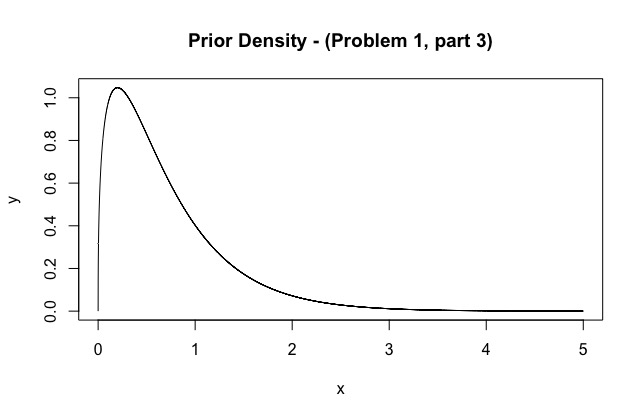
\includegraphics[width=9cm,height=9cm,keepaspectratio]{prob1part3}\\
\begin{lstlisting}{language=R}
> qgamma(.025, 1.4, 2)
[1] 0.04340487
> qgamma(.975, 1.4, 2)
[1] 2.242941
> 0.886*(qgamma(.025, 1.4, 2))^(-1/2)
[1] 4.252698
> 0.886*(qgamma(.975, 1.4, 2))^(-1/2)
[1] 0.5915954
> qgamma(.005, 1.4, 2)
[1] 0.01341205
> qgamma(.995, 1.4, 2)
[1] 3.102909
> 0.886*(qgamma(.005, 1.4, 2))^(-1/2)
[1] 7.650435
> 0.886*(qgamma(.995, 1.4, 2))^(-1/2)
[1] 0.5029782
\end{lstlisting}
From the results we have that
The 95 \% confidence interval is (0.0434, 2.243) and so $E[Y|\theta ] \in (0.592,\ 4.25)$\\
The 99 \% confidence interval is (0.0134, 3.102) and so $E[Y|\theta ] \in (0.503,\ 7.65)$\\
These results satisfy the supposition that gears tend to last between 500 and 5000 hours, y = 0.5 and y = 5, respectively. 
\\\
\\\
\textbf{Part 4}\
The posterior distribution is $$p(\theta|y)=Gamma(n+\alpha, (\sum_{i=1}^{n}y_i^2)+\beta)$$ \\
We are to use a $Gamma(1.4,2)$ prior on $\theta$ and  we know that\\
 $y=(0.25, 0.52, 0.60, 0.91, 0.97, 1.00, 1.07, 1.09, 1.18, 1.38)$,
so \ $n=10$ and $(\sum_{i=1}^{10}y_i^2)=9.0917$.\\
Thus, our posterior is:
$p(\theta|y)=Gamma(n+\alpha, (\sum_{i=1}^{n}y_i^2)+\beta)=Gamma(11.4,11.092)$.\\
The mean of a $Gamma(11.4,11.092)$ is $\mathlarger{\frac{11.4}{11.092} = 1.028}$ and the variance is $\mathlarger{\frac{11.4}{11.092^2}=0.0927}$. \\
R code and plots below.\\
\lstset{backgroundcolor=\color{light-gray}, frame=single, basicstyle = \ttfamily\small}
\begin{lstlisting}{language=R}
> x=seq(0,5,length=10000)
> y=dgamma(x,11.4,11.092)
> plot(x,y, type='l', main='Problem 1 part 4-Posterior density')

> #95% posterior intervals
> qgamma(.025, 11.4, 11.092)
[1] 0.5205005
> qgamma(.975, 11.4, 11.092)
[1] 1.704705
\end{lstlisting}
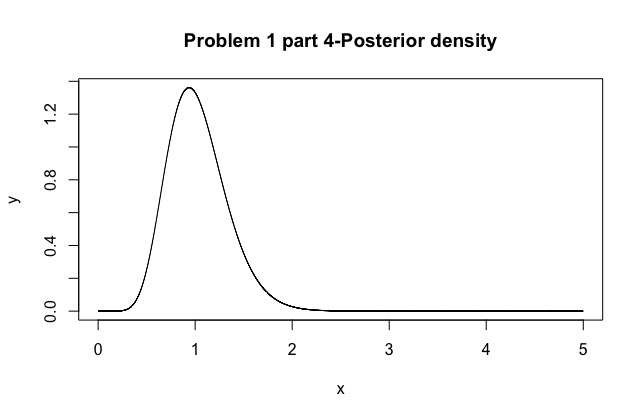
\includegraphics[width=10cm,height=10cm,keepaspectratio]{prob1part4}\\
The 95\% confidence interval for $\theta$ is then (0.521, 1.705).\\
\\\
For the numerical approach, we simulate the posterior in R
\lstset{backgroundcolor=\color{light-gray}, frame=single, basicstyle = \ttfamily\small}
\begin{lstlisting}{language=R}
> x=rgamma(100000,11.4,11.092)
> hist(x)
> mean(x)
[1] 1.028696
> var(x)
[1] 0.09267666
> quantile(x,0.025)
     2.5% 
0.5222731 
> quantile(x,0.975)
   97.5% 
1.705622 
\end{lstlisting}
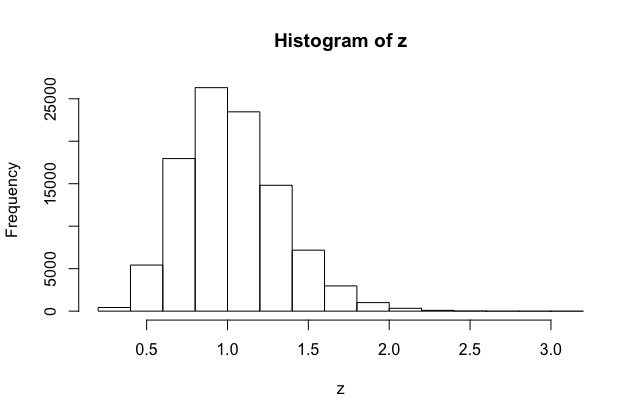
\includegraphics[width=10cm,height=10cm,keepaspectratio]{prob1part4b}
\\\
We see that the histogram, developed numerically, and denisty plot, developed analytically, are very similar. Moreover, the numerical mean was found to be 1.0286 (above) and the variance was found to be 0.0927 (above) which are very similar results compared to the analytical results. The 95\% confidence intervals are also highly similar: The confidence interval found numerically was found to be (0.522,1.706) and the confidence interval found analytically is (0.521, 1.705), which are almost identical.

\section{Problem 2}
\textbf{Part 1}
\newline
We are given a vector of counts $Y = (y_1, y_2, y_3, y_4) = (125, 18, 25, 34)$ where for each $i=1,2,3,4, \ \ y_i$ corresponds to the number of animals observed in the $i^{th}$ category, and $\mathlarger{\sum_{i=1}^4y_i = 202}$. We are further given the corresponding (component-wise) probabilities $\mathlarger{\left(\frac{\theta_1 + \theta_2}{3}, \frac{2(1-\theta_1)}{3}, \frac{1-\theta_2}{3}, \frac{\theta_1}{3}\right)}$ where $\mathlarger{\frac{\theta_1 + \theta_2}{3} + \frac{2(1-\theta_1)}{3} + \frac{1-\theta_2}{3} + \frac{\theta_1}{3} = 1}$. 
\\\
\\\
Then, from Lecture 5 (slide 20), the data likelihood is $$p(y_1, y_2, y_3, y_4 \vert \theta_1, \theta_2) \propto (\frac{1}{3}(\theta_1 + \theta_2))^{y_1}(\frac{2}{3}(1-\theta_1))^{y_2}(\frac{1}{3}(1-\theta_2))^{y_3}(\frac{1}{3}\theta_1)^{y_4} \propto (\theta_1 + \theta_2)^{y_1}(1-\theta_1)^{y_2}(1-\theta_2)^{y_3}\theta_1^{y_4}$$
Since $\theta_1 \sim$ U(0,1) and $\theta_2 \sim$ U(0,1), then assuming independence, $p(\theta_1, \theta_2) = 1$. Then, the posterior is such that\newline
\\\
$p(\theta_1, \theta_2 \vert y_1, y_2, y_3, y_4) \propto (\theta_1 + \theta_2)^{y_1}(1-\theta_1)^{y_2}(1-\theta_2)^{y_3}\theta_1^{y_4}$ .
\\\
\newline
\textbf{Part 2}
\newline
Using the hint, we will augment the parameter vector $(\theta_1,\theta_2)$ to $(\theta_1,\theta_2,z)$ with the probability model:\\
$p(z|y,\theta_1,\theta_2)\sim Bin(y_1,\theta_1/(\theta_1+\theta_2)$
\\\
We then have that,\\
$p(y,z|\theta_1,\theta_2)\propto p(z|y,\theta_1,\theta_2)p(y|\theta_1,\theta_2) \ 
\propto \ \mathlarger{\left(\frac{\theta_1}{\theta_1+\theta_2}\right)^{z}\left(\frac{\theta_2}{\theta_1+\theta_2}\right)^{y_1-z}(\theta_1+\theta_2)^{y_1}(1-\theta_1)^{y_2}(1-\theta_2)^{y_3}\theta_1^{y_4}\  = }\\
\mathlarger{ = \left(\frac{\theta_1^{z}\theta_2^{y_1-z}}{(\theta_1+\theta_2)^{y_1}}\right)(\theta_1+\theta_2)^{y_1}(1-\theta_1)^{y_2}(1-\theta_2)^{y_3}\theta_1^{y_4} = }\\
=\mathlarger{\theta_1^{z+y_4}(1-\theta_1)^{y_2}\theta_2^{y_1-z}(1-\theta_2)^{y_3}
=Beta(\theta_1;z+y_4+1,y_2+1)Beta(\theta_2; y_1-z+1, y_3+1)}$
\\\
\\\
Then,\\
$p(\theta_1,\theta_2|y,z) \propto p(y,z|\theta_2,\theta_2)\pi(\theta_1,\theta_2) \propto Beta(z+y_4+1,y_2+1)Beta(y_1-z+1, y_3+1)$
\\\
From this, we can see that we can use Gibbs sampling to with this data augmentation to simulate the posterior of $(\theta_1,\theta_2)$. 
We will be iterating over values of z (We can start with some initial $(\theta_1^{(0)},\theta_2^{(0)})$ values) :\\
$\mathlarger{z^{(i)} \sim Bin\left( y_1, \ \frac{\theta_1^{(i-1)}}{\theta_1^{(i-1)}+\theta_2^{(i-1)}}\right) = Bin\left(125, \ \frac{\theta_1^{(i-1)}}{\theta_1^{(i-1)}+\theta_2^{(i-1)}}\right)}$\\\
we then generate $(\theta_1,\theta_2)$ as follows:\\
Sample from $p(\theta_1,\theta_2|y,z)$, so \ $\theta_1^{(i)} \sim Beta(z^{(i)}+y_4+1,y_2+1) \ = \ Beta(z^{(i)}+35,19)$ and \\ $\theta_2 \sim Beta(y_1-z^{(i)}+1, y_3+1)\ = \ Beta(126-z^{(i)}, 26)$. \\
We subsequently have a sufficient setup for Gibbs sampling. 
\section{Problem 3}
We are given that the prior distribution on N is geometric with mean 100. That is, \\
$\mathlarger{\pi(N) = \left(\frac{1}{100}\right)\left(\frac{99}{100}\right)^{N-1} = \left(0.01\right)\left(0.99\right)^{N-1}}$ for $N = 1, 2,...$ \\
While N is unknown, we do know that $N \geq 203$, so that the sampling model is given by \[
  p(X = x \vert N) =
  \begin{cases}
                                   \mathlarger{\frac{1}{N}} & \text{, $1\leqslant x \leqslant N$} \\
                                   0 & \text{, otherwise}
  \end{cases} \ \ = \ \begin{cases}
                                   \mathlarger{\frac{1}{N}} & \text{, $N \geq 203$} \\
                                   0 & \text{, otherwise}
  \end{cases} = \ \mathlarger{\frac{1}{N}\times I_{\{N \geq 203\}}}
\]
The posterior is then of the form $p(N\vert X=x) \propto p(X = x\vert N)\pi(N) \propto \mathlarger{\frac{1}{N}\left(0.01\right)\left(0.99\right)^{N-1}\times I_{\{N \geq 203\}}}$.
\\\
\\\
However, if we consider the normalizing constant, we can find the exact form of the posterior distribution, which is required in order to determine the posterior mean and posterior standard deviation.\\
Then, $p(N\vert X=x) = \mathlarger{\frac{1}{p(X)}\frac{1}{N}\left(0.01\right)\left(0.99\right)^{N-1}\times I_{\{N \geq 203\}} = \frac{1}{p(X)}\frac{(0.01)}{(0.99)}\left(\frac{1}{N}(0.99)^N\right) = C\left(\frac{1}{N}(0.99)^N\right)}$ \\
where $C = \mathlarger{\frac{1}{p(X)}\frac{(0.01)}{(0.99)}}$ , a constant.\\
\\\
To determine \ $C$ \ we note that since \ $p(N\vert X=x)$ \ is discrete and $N \geq 203$, we have $$1 = \mathlarger{\sum_{N = 203}^{\infty}p(N\vert X=x) = \ C\sum_{N = 203}^{\infty}\frac{1}{N}(0.99)^N \ \Longrightarrow \ \sum_{N = 203}^{\infty}\frac{1}{N}(0.99)^N = \frac{1}{C}}$$
The infinite sum above was computed in \textit{Mathematica} as follows:
\begin{lstlisting}{language=Mathematica}
In[1]:= Sum[(1/N)*(0.99)^N, {N, 203, Infinity}]

Out[1]= 0.0465803
\end{lstlisting}
Thus, $\mathlarger{\sum_{N = 203}^{\infty}\frac{1}{N}(0.99)^N \ \approx \ 0.0465803 \ \Longrightarrow \ C \approx 21.4683 \ \Longrightarrow \ p(N\vert X = x) \approx 21.4683 \left(\frac{1}{N}(0.99)^N \right)}$\\
Now, $$\mathlarger{E[N\vert X = x] = \sum_{N = 203}^{\infty}Np(N\vert X = x) \ =}$$  $$\mathlarger{ = 21.4683\sum_{N = 203}^{\infty}(0.99)^N \ = \ 21.4683\left(\sum_{N = 0}^{\infty}(0.99)^N - \sum_{N = 0}^{202}(0.99)^N \right) \ =}$$ $$\mathlarger{= \ 21.4683\left(\frac{1}{1 - 0.99} \ - \ \frac{1 - (0.99)^{203}}{1 - 0.99}\right) \ = \ 279.0925397 \  \approx \ 279.093}$$
Now, $\mathlarger{Stdev[N\vert X = x] \ = \ \sqrt{Var[N\vert X = x]} \ = \ \sqrt{E[N^2 \vert X = x] - (E[N \vert X = x])^2}}$ \\
\\\
where, \ 
$E[N^2 \vert X = x] = \mathlarger{\sum_{N = 203}^{\infty}N^2p(N\vert X = x) = 21.4683\sum_{N = 203}^{\infty}N(0.99)^N = 21.4683\left(\frac{(0.99)^{203}(203 - (0.99)(203) + 0.99))}{(1 - 0.99)^2}\right)}$\\
\\\
$ = \ 84284.76918$. \\ (Note: The second-to-last equality uses the identity given in the problem.) \\ 
\\\
Now, \ $\mathlarger{Var[N\vert X = x] \ = \ E[N^2 \vert X = x] - (E[N \vert X = x])^2 \ = \ 84284.76918 - (279.0925397)^2 \ = \ 6392.123461}$\\
$\Longrightarrow \ Stdev(N\vert X = x) \ = \ \sqrt{6392.123461} = 79.95075647 \ \approx \ 79.9508$\\
\\\
Thus, the posterior mean is approximately 279.093 and the posterior standard deviation is approximately 79.9508.

\section{Problem 4}
\textbf{Part 1}\\
We are given the following priors (where $\sigma^{2}_\alpha,a,b $ are known):\\
$p(\sigma_\epsilon^2)=IG(a,b)$\\
$p(\mu)=1$ (flat prior)\\
$p(\alpha_i) = N(0,\sigma^{2}_\alpha) = \mathlarger{ \frac{1}{\sqrt{2\pi\sigma^{2}_\alpha}}e^{-\frac{\alpha^{2}_i}{2\sigma^{2}_\alpha}}} $\\
From the definition of $y_{ij}$, we attain the following conditional distribution:\\
$p(y_{ij}|\mu,\alpha_i,\sigma^{2}_\epsilon) = N(\mu+\alpha_i,\sigma^{2}_\epsilon) = \mathlarger{\frac{1}{\sqrt{2\pi\sigma^{2}_\epsilon}}e^{-\frac{(y_{ij}-\mu-\alpha_i)^2}{2\sigma^{2}_\epsilon}}}$\\
The conditionals for  $\mu,\alpha_i$, and $\sigma^{2}_\epsilon$ are then\\
$\mathlarger{p(\mu|y_{ij},\alpha_i,\sigma^{2}_\epsilon) \propto p(\mu)\prod_{i=1}^{I}\prod_{j=1}^{J}p(y_{ij}|\mu,\alpha_i,\sigma^{2}_\epsilon) 
\propto \prod_{i=1}^{I}\prod_{j=1}^{J}e^{-\frac{(y_{ij}-\mu-\alpha_i)^2}{2\sigma^{2}_\epsilon}} \\
= e^{-\frac{\sum_{i=1}^{I}\sum_{j=1}^{J}(y_{ij}-\mu-\alpha_i)^2}{2\sigma^{2}_\epsilon}} 
\propto e^{-\frac{\sum_{i=1}^{I}\sum_{j=1}^{J}(\mu^{2}-2\mu(y_{ij}-\alpha_i))}{2\sigma^{2}_\epsilon}}}$ \\
$\mathlarger{= e^{-\frac{1}{2\sigma^{2}_\epsilon}(IJ\mu^{2}-2\mu\sum_{i=1}^{I}\sum_{j=1}^{J}(y_{ij}-\alpha_i))} \\
\propto e^{-\frac{IJ}{2\sigma^{2}_\epsilon}(\mu-\frac{\sum_{i=1}^{I}\sum_{j=1}^{J}(y_{ij}-\alpha_i))^2}{IJ}}}$ \ \ \ \ (\textit{by completing the square})\\
$\propto \mathlarger{N\left(\frac{\sum_{i=1}^{I}\sum_{j=1}^{J}(y_{ij}-\alpha_i)}{IJ}, \frac{\sigma^{2}_\epsilon}{IJ}\right)}$\\
\\
Then, \\
$p(\sigma^{2}_\epsilon|y_{ij},\mu,\alpha_i) \propto p(\sigma^{2}_\epsilon)\prod_{i=1}^{I}\prod_{j=1}^{J}p(y_{ij}|\mu,\alpha_i,\sigma^{2}_\epsilon) \\
\propto (\sigma^{2}_\epsilon)^{-a-1}exp(-\frac{b}{\sigma^{2}_\epsilon})(\sigma^{2}_\epsilon)^{-\frac{IJ}{2}}exp(-\frac{\sum_{i=1}^{I}\sum_{j=1}^{J}(y_{ij}-\mu-\alpha_i)^2}{2\sigma^{2}_\epsilon}) \\
\propto (\sigma^{2}_\epsilon)^{-(a+\frac{IJ}{2})-1}exp[-\frac{1}{\sigma^{2}_\epsilon}(b+\frac{1}{2}\sum_{i=1}^{I}\sum_{j=1}^{J}(y_{ij}-\mu-\alpha_i)^2)] \\
\propto IG(a+\frac{IJ}{2},b+\frac{1}{2}\sum_{i=1}^{I}\sum_{j=1}^{J}(y_{ij}-\mu-\alpha_i)^2)$ \ \ \ (\textit{Inverse Gamma})\\
\\
$p(\alpha_i|y_{ij},\mu,\sigma^{2}_\epsilon) \propto p(\alpha_i)\prod_{j=1}^{J}p(y_{ij}|\mu,\alpha_i,\sigma^{2}_\epsilon) \\
\propto exp(-\frac{\alpha^{2}_i}{2\sigma^{2}_\alpha})\prod_{j=1}^{J}exp(-\frac{(y_{ij}-\mu-\alpha_i)^2}{2\sigma^{2}_\epsilon}) \\
= exp[-\frac{\alpha^{2}_i}{2\sigma^{2}_\alpha}-\frac{\sum_{j=1}^{J}(y_{ij}-\mu-\alpha_i)^2}{2\sigma^{2}_\epsilon}] \\
\propto exp[-\frac{\alpha^{2}_i}{2\sigma^{2}_\alpha}-\frac{1}{2\sigma^{2}_\epsilon}(J\alpha^{2}_i-2\sum_{j=1}^{J}\alpha_i(y_{ij}-\mu))] \\
= exp[-\frac{1}{2}((\frac{1}{\sigma^{2}_\alpha}+\frac{J}{\sigma^{2}_\epsilon})\alpha^{2}_i-\frac{2}{\sigma^{2}_\epsilon}\sum_{j=1}^{J}\alpha_i(y_{ij}-\mu))] \\
= exp[-\frac{1}{2}(\frac{1}{\sigma^{2}_\alpha}+\frac{J}{\sigma^{2}_\epsilon})(\alpha^{2}_i-2(\frac{1}{\sigma^{2}_\alpha}+\frac{J}{\sigma^{2}_\epsilon})^{-1}\frac{1}{\sigma^{2}_\epsilon}\sum_{j=1}^{J}\alpha_i(y_{ij}-\mu))] \\
= exp(-\frac{1}{2}(\frac{1}{\sigma^{2}_\alpha}+\frac{J}{\sigma^{2}_\epsilon})(\alpha_i-(\frac{1}{\sigma^{2}_\alpha}+\frac{J}{\sigma^{2}_\epsilon})^{-1}\frac{1}{\sigma^{2}_\epsilon}\sum_{j=1}^{J}(y_{ij}-\mu))^2] \\
\propto N\left(\frac{\sum_{j=1}^{J}(y_{ij}-\mu)}{\sigma^{2}_\epsilon(\frac{1}{\sigma^{2}_\alpha}+\frac{J}{\sigma^{2}_\epsilon})},(\frac{1}{\sigma^{2}_\alpha}+\frac{J}{\sigma^{2}_\epsilon})^{-1}\right)$
\\
\\
\textbf{Part 2}

Gibbs sampling is an example of an MCMC technique. The idea behind these techniques is that we have a Markov chain simulation that converges to some stationary distribution. The important key to this is that the approximate distributions are improved at each iteration of our simulation. An MCMC algorithm has converged at iteration T when its output can be safely thought to arise from the true stationary
distribution of the Markov chain for all t $>$ T. 'Convergence diagnosis' describes tools that help us check whether we have converged to a stationary distribution. One of the tools is a trace plot of the sequence of parameters. This is allows for one to quickly check whether or not the parameters have settled around common values. Another tool is the use of autocorrelation plots. A Markov chain with a high autocorrelation moves around the parameter space slowly, taking it longer to achieve stationarity. High autocorrelation within chains indicate slow mixing and slow convergence. We are
looking for the autocorrelation that significantly decrease over time. Moreover, there are convergence diagnostic statistics (\textit{Source: Geweke, Gelman and Rubin, Heidelberger and Welch, Raftery and Lewis}). \\
If a sample suffers from slow convergence, we can try to run our simulation longer while increasing the thinning interval. We may also try to reparametrize the model. However, care must be taken here because it is possible to overparametrize your model which leads to high posterior correlations among the parameters and slows down the movement of the MCMC sampler through the parameter space. We may also augment the data by adding auxiliary variables. Lastly, we may attempt to "block" correlated variables together in order to speed up convergence. \\
\\
\textbf{Part 3}\\
When we condition on the parameters $\mu$ and $\alpha_i$ being independent and not using any type of hierarchical  centering reparameterizations like in part 4 and part 5 in our ANOVA model, the identifiability of our parameters is weakened. To illustrate this, refer to equation (1):
$$Y_{ij}=\mu+\alpha_i+\epsilon_{ij}$$
It can be seen that this model is overparametrized. Indeed, suppose that $\mu=\pm 1$ and $\alpha_i=\mp 1$ then $Y_{ij} \sim Norm(0,\sigma_\epsilon^2)$. In other words, it is difficult to identify whether $\mu$ or $\alpha_i$ is changing the distribution for $Y_{ij}$. As we stated earlier, this overparameterization leads to high posterior correlations among the parameters and slows down the movement of the MCMC sampler through the parameter space.
\\\
\\\
\textbf{Part 4}\\
From parameterization (i), we have the conditionals that we derived in part 1:\\
$p(\mu|y_{ij},\alpha_i,\sigma^{2}_\epsilon) \sim N(\frac{\sum_{i=1}^{I}\sum_{j=1}^{J}(y_{ij}-\alpha_i)}{IJ}, \frac{\sigma^{2}_\epsilon}{IJ})$\\
$p(\alpha_i|y_{ij},\mu,\sigma^{2}_\epsilon)\sim N(\frac{\sum_{j=1}^{J}(y_{ij}-\mu)}{\sigma^{2}_\epsilon(\frac{1}{\sigma^{2}_\alpha}+\frac{J}{\sigma^{2}_\epsilon})},(\frac{1}{\sigma^{2}_\alpha}+\frac{J}{\sigma^{2}_\epsilon})^{-1})$\\
However, for parameterization (ii), we must derive conditionals for the new parameter:\\
Since $\eta_i=\mu+\alpha_i$, \\
$p(y_{ij}|\mu,\eta_i)= p(y_{ij}|\eta_i) \propto exp(-\frac{1}{2\sigma^{2}_\epsilon}(y_{ij}-\eta_i)^2)$\\
$p(\eta_i|\mu) \propto exp(-\frac{1}{2\sigma^{2}_\alpha}(\eta_i-\mu)^2)$.\\
We want $p(\mu|y_{ij},\eta_i)$ and $p(\eta_i|y_{ij},\mu)$. Then, \\
$p(\mu|y_{ij},\eta_i) \propto \prod_{i=1}^{I}p(\eta_i|\mu) \propto exp(-\frac{1}{2\sigma^{2}_\alpha}\sum_{i=1}^{I}(\eta_i-\mu)^2) \\
\propto exp[-\frac{1}{2\sigma^{2}_\alpha}(I\mu^2-2\mu\sum_{i=1}^{I}\eta_i)]  \\
= exp[-\frac{1}{2\sigma^{2}_\alpha/I}(\mu^2-\frac{2\mu}{I}\sum_{i=1}^{I}\eta_i)]  \\
\propto exp[-\frac{1}{2\sigma^{2}_\alpha/I}(\mu-\frac{1}{I}\sum_{i=1}^{I}\eta_i)^2]  \\
\propto N(\frac{\sum_{i=1}^{I}\eta_i}{I}, \frac{\sigma^{2}_\alpha}{I})$\\
\\
$p(\eta_i|y_{ij},\mu) \propto \prod_{j=1}^{J}p(y_{ij}|\eta_i)p(\eta_i|\mu) 
\propto exp(-\frac{1}{2\sigma^{2}_\epsilon}\sum_{j=1}^{J}(y_{ij}-\eta_i)^2)exp(-\frac{1}{2\sigma^{2}_\alpha}(\eta_i-\mu)^2) \\
= exp(-\frac{1}{2\sigma^{2}_\epsilon}\sum_{j=1}^{J}(y_{ij}-\eta_i)^2-\frac{1}{2\sigma^{2}_\alpha}(\eta_i-\mu)^2) \\
\propto exp(-\frac{1}{2\sigma^{2}_\epsilon}(J{\eta_i}^2-2\eta_i\sum_{j=1}^{J}y_{ij})-\frac{1}{2\sigma^{2}_\alpha}({\eta_i}^2-2\eta_i\mu))  \\
\propto exp[-\frac{1}{2}((\frac{1}{\sigma^{2}_\alpha}+\frac{J}{\sigma^{2}_\epsilon}){\eta_i}^2-2\eta_i(\frac{\mu}{\sigma^{2}_\alpha}+\frac{1}{\sigma^{2}_\epsilon}\sum_{j=1}^{J}y_{ij}))]  \\
\propto exp[-\frac{1}{2}(\frac{1}{\sigma^{2}_\alpha}+\frac{J}{\sigma^{2}_\epsilon})(\eta_i-(\frac{1}{\sigma^{2}_\alpha}+\frac{J}{\sigma^{2}_\epsilon})^{-1}(\frac{\mu}{\sigma^{2}_\alpha}+\frac{1}{\sigma^{2}_\epsilon}\sum_{j=1}^{J}y_{ij}))^2]  \\
\propto N((\frac{1}{\sigma^{2}_\alpha}+\frac{J}{\sigma^{2}_\epsilon})^{-1}(\frac{\mu}{\sigma^{2}_\alpha}+\frac{1}{\sigma^{2}_\epsilon}\sum_{j=1}^{J}y_{ij}),(\frac{1}{\sigma^{2}_\alpha}+\frac{J}{\sigma^{2}_\epsilon})^{-1})$\\
Now, using the Gibbs sampler for these two parameterizations we can investigate their autocorrelations.\\
(\textit{R code and output below})
\\\
\textbf{R code:}
\lstset{backgroundcolor=\color{light-gray}, frame=single, basicstyle = \ttfamily\small}
\begin{lstlisting}{language=R}
I=5
J=1
sigma.a=1
sigma.e=1
B=1000  #burnout period
N=10000
alpha=matrix(0,I,N+B)
alpha[,1]=numeric(I)
mu1=numeric(N+B)
mu1[1]=0

#Generating data from (1)
Y=matrix(0,I,J)
for (i in 1:I){
  alpha.i=rnorm(n=1,0,sigma.a)
  for (j in 1:J){
    Y[i,j]=rnorm(n=1,alpha.i,sigma.e)
  }
}
#Gibbs sampler for parameterization(i):
for (k in 2:(B+N)){
  x=matrix(0,I,J)
  for (i in 1:I){
    for (j in 1:J){
      x[i,j]=Y[i,j]-(alpha[i,k-1])
    }
  }
  new=sum(x)/(I*J)
  mu1[k]=rnorm(n=1,new,sigma.e/sqrt(I*J))
  for (i in 1:I){
    sigma.i=sqrt((J/sigma.e^2+1/sigma.a^2)^(-1))
    mu1.i=sum(Y[i,]-mu1[k])/sigma.e^2*sigma.i^2
    alpha[i,k]=rnorm(1,mu1.i,sigma.i)
  }
}
#Gibbs sampler or parameterization(ii) :
mu2=numeric(N+B)
mu2[1]=0
e=matrix(0,I,B+N)
e[,1]=numeric(I)
for (k in 2:(B+N)){
  mu2[k]=rnorm(n=1,mean(e[,k-1]),sigma.a/sqrt(I))
  for (i in 1:I){
    sigma.i=sqrt((J/sigma.e^2+1/sigma.a^2)^(-1))
    mu1.i=(sum(Y[i,])/sigma.e^2+mu2[k]/sigma.a^2)*
      sigma.i^2
    e[i,k]=rnorm(1,mu1.i,sigma.i)
  }
}
#Investigation of the sample ACF
acf(mu1[(B+1):(B+N)], main="Sample ACF for mu - parametrization (i) (Part 4)")
acf(alpha[1,(B+1):(B+N)], main="Sample ACF for alpha - parametrization (i), (Part 4)")
acf(mu2[(B+1):(B+N)], main="Sample ACF for mu - parametrization (ii), (Part 4)")
acf(e[1,(B+1):(B+N)], main="Sample ACF for eta - parametrization (ii), (Part 4)")

\end{lstlisting}
\textbf{Outputs and ACF Plots:}\\
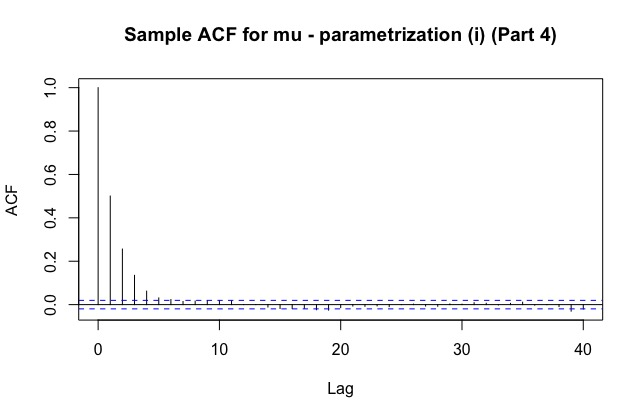
\includegraphics[width=9cm,height=9cm,keepaspectratio]{part4mu1}
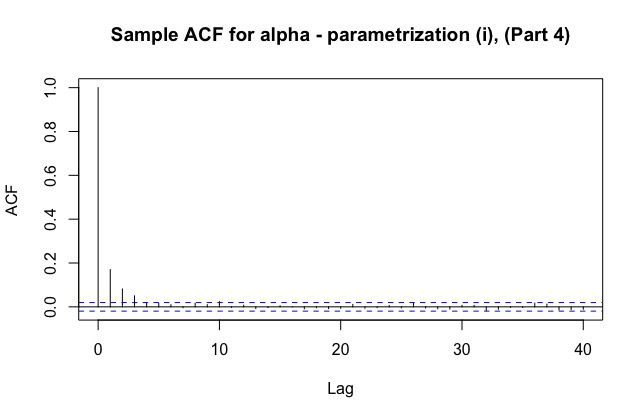
\includegraphics[width=9cm,height=9cm,keepaspectratio]{part4alpha1}
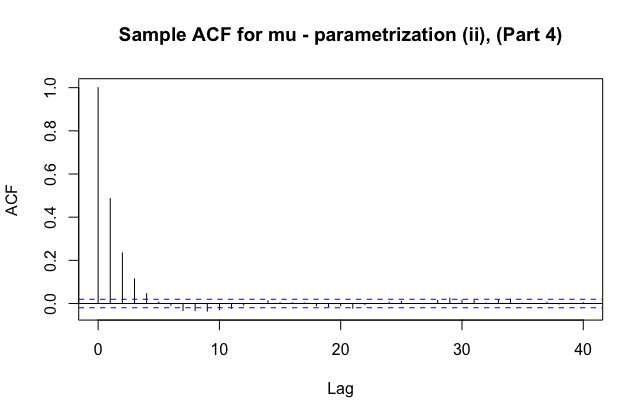
\includegraphics[width=9cm,height=9cm,keepaspectratio]{part4mu2}
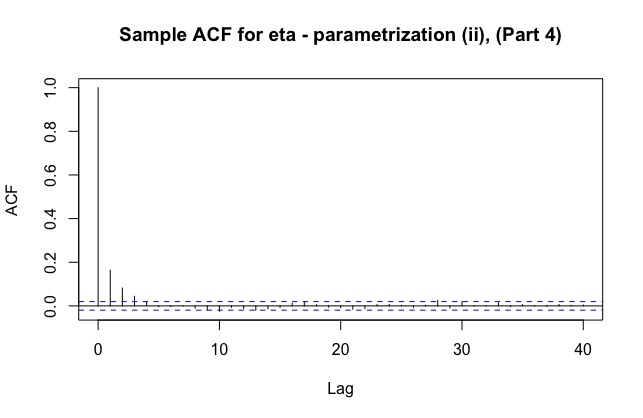
\includegraphics[width=9cm,height=9cm,keepaspectratio]{part4eta}\\
Upon investigation of the ACF plots for both parameterizations, there does not seem to be any significant differences between them. Both ACF plots tail off rather quickly around similar lag times. This implies that when when $\sigma_\alpha^2=\sigma_\epsilon^2=1$, neither of the two parameterizations significantly outperforms the other. \\
\\\
\textbf{Part 5}\\
We are going to rerun the program from Part 4, but for the case $\sigma_\alpha^2=10$ and $\sigma_\epsilon^2=1$.
\\\
\textbf{R Code:}
\lstset{backgroundcolor=\color{light-gray}, frame=single, basicstyle = \ttfamily\small}
\begin{lstlisting}{language=R}
I=5
J=1
sigma.a=sqrt(10)
sigma.e=1
B=1000 #Burnout period
N=10000
alpha=matrix(0,I,N+B)
alpha[,1]=numeric(I)
mu1=numeric(N+B)
mu1[1]=0

#Generating data from (1)
Y=matrix(0,I,J)
for (i in 1:I){
  alpha.i=rnorm(n=1,0,sigma.a)
  for (j in 1:J){
    Y[i,j]=rnorm(n=1,alpha.i,sigma.e)
  }
}
#Gibbs sampler for parameterization(i) :
for (k in 2:(B+N)){
  x=matrix(0,I,J)
  for (i in 1:I){
    for (j in 1:J){
      x[i,j]=Y[i,j]-(alpha[i,k-1])
    }
  }
  new=sum(x)/(I*J)
  mu1[k]=rnorm(n=1,new,sigma.e/sqrt(I*J))
  for (i in 1:I){
    sigma.i=sqrt((J/sigma.e^2+1/sigma.a^2)^(-1))
    mu1.i=sum(Y[i,]-mu1[k])/sigma.e^2*sigma.i^2
    alpha[i,k]=rnorm(1,mu1.i,sigma.i)
  }
}
#Gibbs sampler for parameterization(ii) :
mu2=numeric(N+B)
mu2[1]=0
e=matrix(0,I,B+N)
e[,1]=numeric(I)
for (k in 2:(B+N)){
  mu2[k]=rnorm(n=1,mean(e[,k-1]),sigma.a/sqrt(I))
  for (i in 1:I){
    sigma.i=sqrt((J/sigma.e^2+1/sigma.a^2)^(-1))
    mu1.i=(sum(Y[i,])/sigma.e^2+mu2[k]/sigma.a^2)*
      sigma.i^2
    e[i,k]=rnorm(1,mu1.i,sigma.i)
  }
}
#Investigation of the sample ACF
acf(mu1[(B+1):(B+N)], main="Sample ACF for mu - parametrization (i), (Part 5)")
acf(alpha[1,(B+1):(B+N)], main="Sample ACF for alpha - parametrization (i), (Part 5)")
acf(mu2[(B+1):(B+N)], main="Sample ACF for mu - parametrization (ii), (Part 5)")
acf(e[1,(B+1):(B+N)], main="Sample ACF for eta - parametrization (ii), (Part 5)")
\end{lstlisting}
\textbf{Output and ACF Plots:}\\
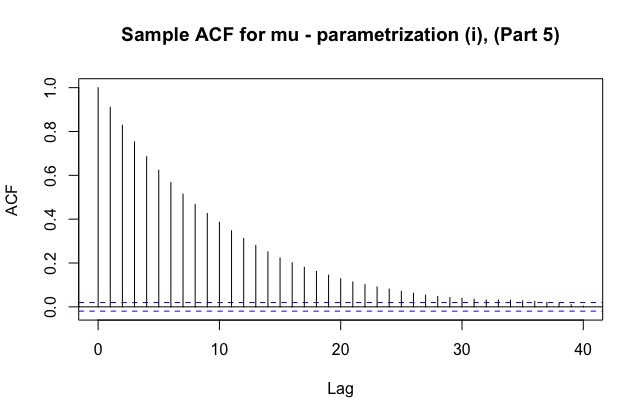
\includegraphics[width=9cm,height=9cm,keepaspectratio]{part5mu1}
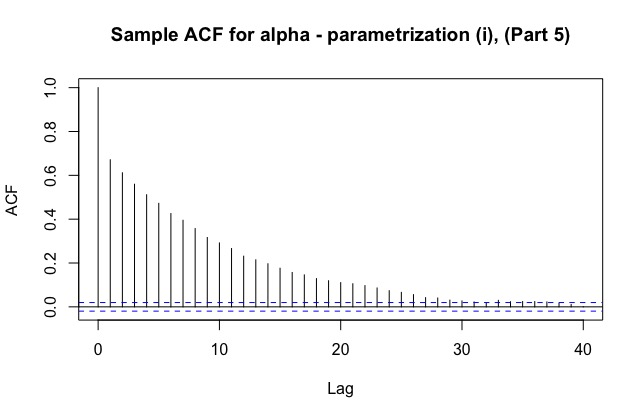
\includegraphics[width=9cm,height=9cm,keepaspectratio]{part5alpha1}
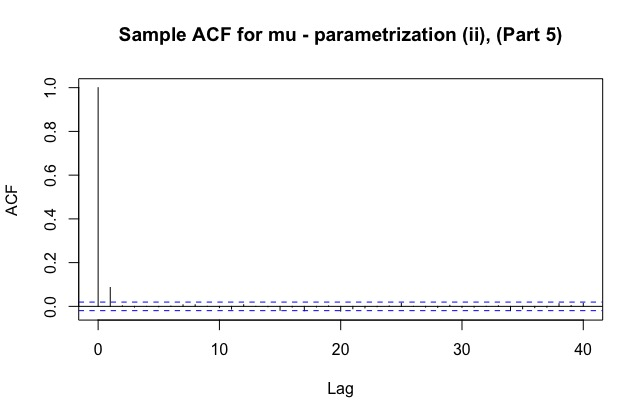
\includegraphics[width=9cm,height=9cm,keepaspectratio]{part5mu2}
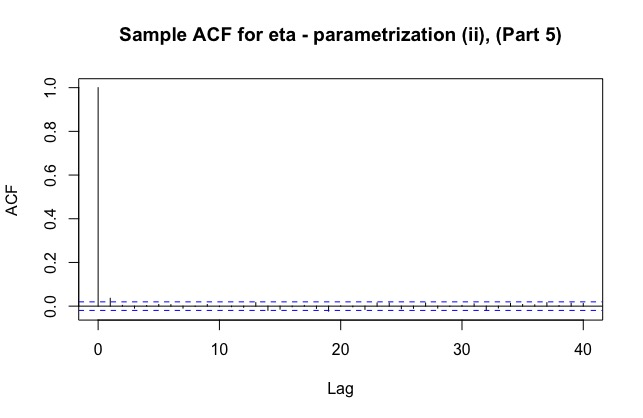
\includegraphics[width=9cm,height=9cm,keepaspectratio]{part5eta}\\
After investigating the ACF plots for this case, it can be seen (above) that the ACF plots for parameterization(ii) tail off significantly faster for each parameter, $\mu$ and 
$\eta$, compared to the ACF plots for parameterization(i). This implies that parameterization(ii) converges faster, thus outperforming parameterization(i). Consequently, these results can lead us to conclude that hierarchical centering reparametrizations can potentially resolve issues with 
identifiability in overparameterized models, resulting in much faster convergence rates toward a stationary distribution. 
\section{Problem 5}
\textbf{Part 1}
\newline
We are given a hypothetical situation where the distance between the two school districts is so far that the school districts share no similarities, so it is reasonable to use an independent prior for $\theta_1$ and $\theta_2$. Since the $\theta_i$'s correspond to exam scores, and if we assume a \ 0 - 100 grading scale (we can always normalize the scale to 0 - 100 if it isn't), it's reasonable to use a prior mean of 50, where we are given that the prior variance is 16 (so the variance is known). We will also suppose that $\theta_i$ is normally distributed (a normal prior), for $i = 1, 2$, so that $\theta_i \sim N(50, 16)$. Since we are using an independent prior for $\theta_1$ and $\theta_2$, our joint prior is $\pi(\theta_1, \theta_2)$ = $\pi(\theta_1)\pi(\theta_2)$ where $\pi(\theta_i)$ is a normal distribution with mean $\mu_0 = 50$ and variance $\sigma_0^2 = 16$, for $i = 1, 2$. That is, we have independent conjugate priors.\\
We are also given that $\bar{y_1}\vert\theta_1 \sim N(\theta_1, \ \frac{14}{8})$ and $\bar{y_2}\vert\theta_2 \sim N(\theta_2, \ \frac{14}{24})$\\ 
From Hoff (and from lecture), we know that with known variance, if $x \vert \mu \sim N(\mu, \sigma^2)$ and $\mu \sim N(\mu_0, \sigma_0^2)$, then the posterior is given by $\mu\vert x \sim N(\frac{\sigma_0^2}{\sigma^2+\sigma_0^2}y+\frac{\sigma^2}{\sigma^2+\sigma_0^2}\mu_0,(\frac{1}{\sigma_0^2}+\frac{1}{\sigma^2})^{-1})$. Then, in our case, since the variance is known and we have independent conjugate priors and independent, identically distributed sampling models\\
$\mathlarger{(\theta_1\vert \bar{y_1} = 40) \sim N\left(\frac{16}{14/8+16}(40)+\frac{14/8}{14/8+16}(50), \ (\frac{1}{16}+\frac{1}{14/8})^{-1}\right)=N(40.986, \ 1.577)}$ and \\
$\mathlarger{(\theta_2\vert \bar{y_2} = 26) \sim N\left(\frac{16}{14/24+16}(26)+\frac{14/24}{14/24+16}(50), \ (\frac{1}{16}+\frac{1}{14/24})^{-1}\right)=N(26.844, \ 0.563)}$ \\
\\\
Thus, our Bayesian estimate for $\theta_1$ is 40.986 with standard deviation $\sqrt{1.577} = 1.256$. The Bayesian estimate for $\theta_2$ is 26.844 with standard deviation $\sqrt{0.563} = 0.750$.
\begin{flushleft}
\textbf{Part 2}
\end{flushleft}
Here, the situation is that the school districts are adjacent to each other implying similarity. It is then reasonable to use a dependent prior for $\theta_1$ and $\theta_2$. In particular, suppose that $(\theta_1, \theta_2)$ is jointly normally distributed, that is $(\theta_1, \theta_2) \sim N(\mu, \Sigma)$. Similar to part 1, let $\mu = [50, 50]^T$ and since we are given a variance of 16, let
$\Sigma=\begin{bmatrix}
16 & 8\\
8  & 16\\
\end{bmatrix}$\\
We then have that $\overline{y}=[\overline{y_1},\overline{y_2}]^T$ also follows a multivariate normal distribution. In particular, $\overline{y} \sim N(\theta, D)$ \ 
where $\theta=[\theta_1,\theta_2]^T$ and $D=\begin{bmatrix}
14/n_1 & 0\\
0  & 14/n_2\\
\end{bmatrix}=\begin{bmatrix}
14/8 & 0\\
0  & 14/24\\
\end{bmatrix}$\\
Since the multivariate normal distribution is the conjugate prior for the multivariate normal distribution, our posterior distribution is multivariate normal. Then,\\
$\theta_1,\theta_2|y \sim N(\mu^*,\Sigma^*)$,
where:
$(\Sigma^*)^{-1}=\Sigma^{-1}+D^{-1}$
and
$\mu^*=\Sigma^*(\Sigma^{-1}\mu+D^{-1}\overline{y})
$\\
After a bit of computation, it was found that:\\
$\mu^*=[39.80,26.87]^T\\
\\\
\Sigma^*=\begin{bmatrix}
1.53 & 0.036\\
0.036  & 0.57\\
\end{bmatrix}$\\
\\
(our Bayesian estimates)
\\\
\textbf{Part 3}\\
In part 1, we used an independent prior to represent the lack of similarity between the two districts while in part 2 we used an MVN prior and assumed that the covariance between $\theta_1$ and $\theta_2$ was half the variance (> 0), so we used a dependent prior. Parts 1 and 2 were similar in that we used a prior mean of 50 for both district 1 and 2. What is very interesting is that the Bayesian estimates and the corresponding variances in parts 1 and 2 are very similar:\\
\begin{table}[h]
\centering
\begin{tabular}{c c c}
\hline\hline
& \ \ $\theta_1$ & $\theta_2$ \\
\hline\hline
Part 1 Bayesian Estimates & \ \ 40.99 & \ 26.84 \\ 
\hline
Part 2 Bayesian Estimates & \ \ 39.80 & \ 26.87  \\  
\hline
Part 1 Variance & \ \ 1.58 & \ 0.56 \\
\hline
Part 2 Variance & \ \ 1.53 & \ 0.57 \\
\hline\hline
\end{tabular}
\label{tab:hresult}
\end{table}

While the Bayesian estimates for parts 1 and 2 are similar, there is a bit of difference. Because the covariance in part 2 is non-zero, whereas it is 0 in part 1 (since independent), the Bayesian estimate (posterior mean) for district 1 is less than the sample mean (= 40), while the estimate (posterior mean) for district 1 in part 1 is greater than the sample mean (= 40). 
Also notice that the posterior covariance in part 2 is very small, 0.0036; however, this is not too surprising considering the assumed sampling distribution for $\overline{y}_i$ - which is the same sampling distribution used in part 1 and part 2.
\section{Problem 6}
\textbf{Part 1} \\
We are given that model $H_1$ is such that \ $\beta_1 \sim N(0,1), \ \beta_2 \sim N(1,1) $\\
and model $H_2$ is such that \ $\gamma_1 \sim N(0,1), \ \gamma_2 \sim N(1,1), \ \gamma_3 \sim N(0,1) $\\
where, in each part, the parameters are a \textit{priori} independent, which implies that the joint distributions are multivariate normal with the identity matrix equal to the covariance matrix. \\
To make the computations less messy, we should compactify our data into matrices: \\
Let \ $X_1=\begin{bmatrix}
1&x_1\\
1&x_2\\
\vdots&\vdots\\
1&x_i
\end{bmatrix}$ , \ \ \ \ 
$X_2=\begin{bmatrix}
1&x_1&x_1^2\\
1&x_2&x_2^2\\
\vdots&\vdots&\vdots\\
1&x_i&x_i^2
\end{bmatrix}$, \ \ $\mu_1=[0 \ 1]^T$, \ \ $\mu_2=[0 \ 1 \ 0]^T$ \\
\\\
$y=[y_1, ...y_n]^T, x=[x_1,...x_n]^T, \beta=[\beta_1,\beta_2]^T, \gamma=[\gamma_1,\gamma_2,\gamma_3]^T $. \\
\\\
We then have $p(y|\beta)=N(X_1\beta,I)$ \ and \ $p(\beta)=N(\mu_1,I)$ where $I$ is the identity matrix. \\
Observe that:\\
$p(X_1\beta)=N(X_1\mu_1,X_1IX_1^T)=N(X_1\mu_1,X_1X_1^T)$\\
We may now compute $p(y|H_1)$:\\
$p(y|H_1)=\int p(y|\beta)p(\beta)d\beta= \int N(X_1\beta,I)N(\mu_1,I)d\beta\\
=N(X_1\mu_1,I+X_1 X_1^T)$\\
Similarly,\\
$p(y|H_2)=\int p(y|\gamma)p(\gamma)d\gamma= \int N(X_2\gamma,I)N(\mu_2,I)d\gamma\\
=N(X_2\mu_2,I+X_2 X_2^T)$\\
\\
\textbf{Part 2} \\
From the results of part 1, we can simply plug our data set into the constructed matrices $X_1$ and $X_2$, where we obtain the Bayes factor:\\
\\\
$B=\dfrac{p(y|H_2)}{p(y|H_1)}=\dfrac{N(X_2\mu_2,I+X_2 X_2^T)}{N(X_1\mu_1,I+X_1 X_1^T)}
=\dfrac{(2\pi)^{-\frac{n}{2}}(|I+X_2 X_2^T|)^{-\frac{1}{2}}exp[-\frac{1}{2}(y-\mu_2)^T(I+X_2 X_2^T)^{-1}(y-\mu_2)]}{(2\pi)^{-\frac{n}{2}}(|I+X_1 X_1^T|)^{-\frac{1}{2}}exp[-\frac{1}{2}(y-\mu_1)^T(I+X_1 X_1^T)^{-1}(y-\mu_1)]}\\
\\\
 \approx 0.34$\\
\\
\textbf{Part 3}
\begin{proof}
We are given that $p(\beta)=c_1$, $p(\gamma)=c_2$. It then follows that
$$\mathlarger{p(y|H_1) = \int p(y|\beta)p(\beta)d\beta = \int c_1 N(y|X_1\beta,I) d\beta = \int c_1 (2\pi)^{-\frac{n}{2}}e^{-\frac{1}{2}(y-X_1\beta)^T(y-X_1\beta)} d\beta =}$$ $$\mathlarger{ = c_1 (2\pi)^{-\frac{n}{2}}\int e^{-\frac{1}{2}(y^Ty-2\beta^TX_1^Ty+\beta^TX_1^TX_1\beta)}d\beta = }$$ $$\mathlarger{ = c_1 (2\pi)^{-\frac{n}{2}}e^{-\frac{1}{2}y^Ty} \int e^{-\frac{1}{2}(\beta^TX_1^TX_1\beta-2\beta (X_1^TX_1) (X_1^TX_1)^{-1}X_1^Ty )}d\beta}$$
Now let $\hat{\beta}=(X_1^TX_1)^{-1}X_1^Ty$ (similar to an Ordinary Least Squares estimate!)\\
$$\mathlarger{p(y|H_1)=c_1 (2\pi)^{-\frac{n}{2}}e^{-\frac{1}{2}y^Ty} \int e^{-\frac{1}{2}(\beta^TX_1^TX_1\beta-2\beta (X_1^TX_1)\hat{\beta}+\hat{\beta}^T(X_1^TX_1)\hat{\beta} )}d\beta \cdot e^{\frac{1}{2}\hat{\beta}^T(X_1^TX_1)\hat{\beta}} =}$$ $$\mathlarger{ = c_1 (2\pi)^{-\frac{n}{2}} e^{-\frac{1}{2}y^Ty+\frac{1}{2}\hat{\beta}^T(X_1^TX_1)\hat{\beta}}\times|(X_1^TX_1)|^{-\frac{1}{2}}}$$\\
By the same argument,\\
$$\mathlarger{p(y|H_2)=\int p(y|\gamma)p(\gamma)d\gamma =c_2 (2\pi)^{-\frac{n}{2}} e^{-\frac{1}{2}y^Ty+\frac{1}{2}\hat{\gamma}^T(X_2^TX_2)\hat{\gamma}}\times|(X_2^TX_2)|^{-\frac{1}{2}}}$$\\
We are now prepared to compute the Bayes factor:\\
\\\
$$\mathlarger{\widetilde{B}=\dfrac{\int p(y|\gamma)p(\gamma)d\gamma}{\int p(y|\beta)p(\beta)d\beta} \ = \ \dfrac{c_2 (2\pi)^{-\frac{n}{2}} e^{-\frac{1}{2}y^Ty+\frac{1}{2}\hat{\gamma}^T(X_2^TX_2)\hat{\gamma}}\times|(X_2^TX_2)|^{-\frac{1}{2}}}{c_1 (2\pi)^{-\frac{n}{2}} e^{-\frac{1}{2}y^Ty+\frac{1}{2}\hat{\beta}^T(X_1^TX_1)\hat{\beta}}\times|(X_1^TX_1)|^{-\frac{1}{2}}}} \ =$$ $$\mathlarger{ = \ \dfrac{(c_2) e^{\frac{1}{2}\hat{\gamma}^T(X_2^TX_2)\hat{\gamma}}\times|(X_2^TX_2)|^{-\frac{1}{2}}}{(c_1)  e^{\frac{1}{2}\hat{\beta}^T(X_1^TX_1)\hat{\beta}}\times|(X_1^TX_1)|^{-\frac{1}{2}}}}$$
$\Longrightarrow \ \ \widetilde{B} \mathlarger{ = \ \dfrac{(c_2) e^{\frac{1}{2}\hat{\gamma}^T(X_2^TX_2)\hat{\gamma}}\times|(X_2^TX_2)|^{-\frac{1}{2}}}{(c_1)  e^{\frac{1}{2}\hat{\beta}^T(X_1^TX_1)\hat{\beta}}\times|(X_1^TX_1)|^{-\frac{1}{2}}}}$\\
\\\
From this, it is clear that the value of the Bayes factor $\widetilde{B}$ depends on the arbitrarily chosen constants $c_1$ and $c_2$.
\end{proof}
\end{document}